\section{Mediciones sobre el prototipo}

[VER SI ESTÁ BIEN SEPARAR EN IMPLEMENTACIÓN Y MEDICIONES O HACERLO TODA UNA MISMA SECCIÓN]

Como se mencionó previamente, el objetivo del prototipo era verificar el correcto funcionamiento del circuito real. Para eso la etapa de medición es crucial, dado que se puede utilizar para buscar posibles errores y mejoras a implementar en el dispositivo final. Sin embargo, como medida cortafuegos, se decidió soldar el prototipo y medir de forma progresiva: primero una celda, luego un banco, y finalmente todo el circuito. De este modo, en caso de haber alguna falla crítica, se puede detectar de forma temprana antes de ya haber dedicado más trabajo y usado todos los componentes a disposición.

\subsection{Primera medición fallida en una celda del banco 1}

Lo primero que se soldó fue el circuito de una de las celda junto con la etapa de control del banco $1$. Aunque a simple vista parecía que todo estaba en orden, rápidamente se reveló que no era el caso.

[INSERTAR IMAGEN DEL KICAD Y FOTO DE ESTA CELDA]

En primer lugar se buscó verificar el funcionamiento en estado estacionario de la celda, por lo que se conectó a la entrada una fuente de tensión continua de \SI{5}{\volt} (con una corriente de hasta \SI{20}{\milli\ampere}). Esto debería ser suficiente para obtener como tensión de salida a la de la celda pero no fue el caso: la salida era nula con pequeñas variaciones ocasionales en torno a las decenas de milivolts.

Ante la temprana falla se midieron las caídas de tensión de todos los componentes en las mallas de control. Cuando se estaba midiendo la caída sobre el resistor $R_3$, el TBJ PNP $Qij_2$ comenzó a soltar humo. De este punto en adelante se desataron una serie de eventos desafortunados que concluyeron en el reemplazo de varios componentes más.

En el intento de desoldar el transistor para reemplazarlo, el diodo \textit{zener} también empezó a soltar humo. Fue tanta la temperatura que desprendió que el estaño que lo sujetaba se fundió. Cabe destacar que la fuente de continua no estaba conectada pero sí estaba colocada la celda. Aunque debido a la baja potencia que emite, ésta no debería haber sido la causa de la destrucción del diodo.

Luego, más humo se desprendió de lo que parecería ser el fusible de la celda. Éste fue rápidamente extraído, aunque luego de unas pruebas con multímetro se descubrió que ambos fusibles estaban perfectamente bien y que ninguno se había quemado.

Dado este nuevo suceso, se decidió que lo más probable que se haya quemado era el transitor N-MOSFET de la tierra, por lo que se lo desoldó. Debido a la proximidad con otros componentes, el calor del soldador fue tal que el plástico del portafusible de la celda se derritió. No hubo otra opción que también descartarlo, siendo el cuarto componente en seguidilla en ser eliminado y sin tener una clara idea de cuál fue el problema.

\subsection{Segundo intento de medición y primero exitoso}

Luego de los problemas del intento anterior, se priorizó restaurar los componentes en la placa, asegurándose en cada paso el correcto funcionamiento de los mismos. Comenzando por la etapa de control, se soldaron nuevos TBJ NPN y diodo \textit{zener}. Ingresando una tensión de control equivalente a un $1$ lógico (\SI{5}{\volt}) se corroboró la correcta apertura del transistor.

Luego, debido a la proximidad de los componentes y el gran tamaño relativo de los portafusibles, se decidió extraerlos. En su lugar se colocaron alambres para cerrar las mallas en las que estaban colocados.

Con lo soldado hasta ahora el sistema debería prender y apagar correctamente la celda. Lo único faltante es el N-MOSFET de la tierra. Cuando se lo desoldó, la pista quedó dañada y se soltó el \textit{pad}, por lo que colocarlo nuevamente resultaría dificultoso. Más adelante es algo que debe hacerse (y se hizo) pero por el momento se podría medir sin el transistor y cortocircuitar la tierra con el nodo correspondiente de forma manual con cables cuando sea necesario.

Con el circuito de la celda devuelto a casi su estado original se conectó todo para volver a medir. Cabe destacar que en lugar de la celda de litio se colocó una tensión a través de una fuente de continua. La razón detrás de esta decisión fue colocar una corriente máxima de \SI{100}{\milli\ampere} para, en caso de que algo falle, minimizar la probabilidad de quemar más componentes.

Con todo esto en mente, se encendieron las fuentes que emiten la tensión de la celda y la entrada de control y se obtuvo a la salida la tensión de la celda. Aunque un progreso respecto del último intento de medición, rápidamente se hizo notorio otro problema: la fuente de la celda estaba emitiendo corriente. Normalmente eso es lo que se esperaría ver salvo cuando la salida está abierta (como era el caso en cuestión) donde no debería haber corriente circulando. Estos valores rondaban los \SI{80}{\milli\ampere} o \SI{90}{\milli\ampere}, valores para nada despreciables. 

Midiendo la caída de tensión en cada componente se encontró la ubicación del problema: había caída de tensión en los resistores $R_7$ y $R_8$ correspondientes a la etapa de control del \textit{switch} del banco. En ellos caían [PONER VALOR TENSIONES].

[AGREGAR IMAGEN CON EL REDONDEL ROJO DE LOS RESISTORES EN CUESTIÓN]

Ese bloque estaba apagado por lo que no debería haber corriente circulando por sus componentes. Testeando continuidad en el nodo de [LA FIGURA QUE FALTA ARRIBA] hay un cortocircuito con tierra. Se desoldó el TBJ, el cual se partió a la mitad. Probablemente haya estado quemado, lo cual explicaría el humo visto previamente en el primer intento de medición que se había creído erróneamente que provenía de alguno de los fusibles. El cortocircuito seguía estando por lo que también se extrajo el JFET, momento en el cual se solucionó el problema.

Nuevamente se incorporan las fuente de tensión y esta vez sí se obtiene el resultado esperado: \SI{33.}{\volt} a la salida con corriente nula. Incorporando cargas de prueba se aprecia que la corriente de salida varía. El MOSFET de la tierra flotante sigue ausente pero se pudo corroborar el correcto funcionamiento del encendido y apagado de una celda.

\subsection{Problemas de diseño del prototipo}

Entre mediciones fallidas y valores no esperados, se pudieron identificar algunos errores de diseño. Por un lado por huellas mal elegidas, y por otro, por errores en el esquemático. Antes de detallarlos es importante destacar que ninguno de estos problemas son críticos ni inhibieron el circuito. Aunque simples de corregir para la versión final, requirieron de trabajo y tiempo al momento de identificarlos.

En primer lugar se tienen los problemas en las huellas, comenzando por la de los JFET. Debido a una confusión con los TBJ, los cuales usan el mismo encapsulado pero diferente configuración de los pines, la huella en \textit{KiCad} no coincidió con la dada en la \textit{datasheet}, como se muestra en la figura \ref{fig:JFET_pinout}.

\begin{figure}[H]
    \centering
    \begin{subfigure}{0.3\textwidth}
        \centering
        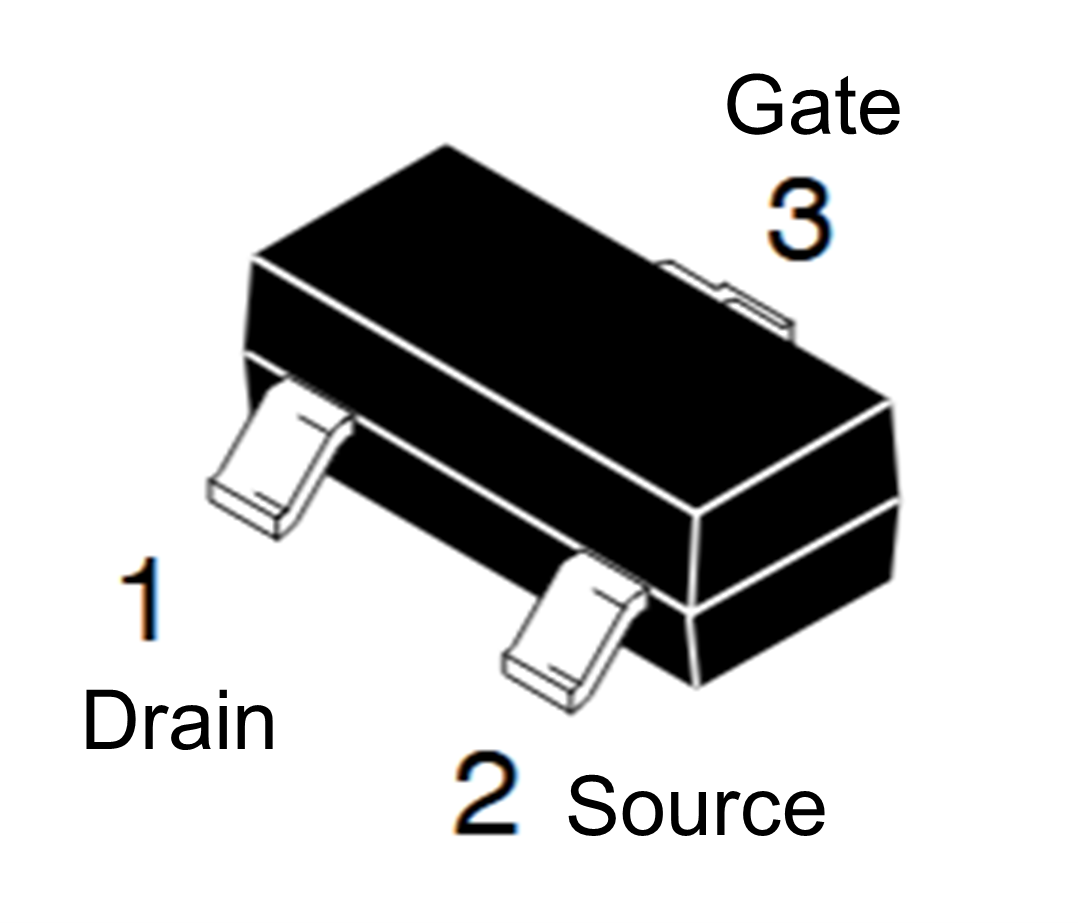
\includegraphics[width=\linewidth]{Imágenes/Prototipo/JFET pines con nombre.png}
        \caption{}
        \label{fig:JFET_pinout_datasheet}
    \end{subfigure}
    \hfill
    \begin{subfigure}{0.4\textwidth}
        \centering
        
\includegraphics[width=\linewidth]{Imágenes/Prototipo/JFET pines con nombre KiCad.png}
        \caption{}
        \label{fig:JFET_pinout_kicad}
    \end{subfigure}
    \caption{\textit{Pinout} del JFET MMBFJ201 según la hoja de datos (a) y como fue configurado en la huella de \textit{KiCad} (b).}
    \label{fig:JFET_pinout}
\end{figure}

De forma similar, la huella de los diodos \textit{zener} estaba invertida. Esto significó una inversión del ánodo y el cátodo como se aprecia en la figura \ref{fig:zener_kicad}.

\begin{figure}[H]
    \centering
    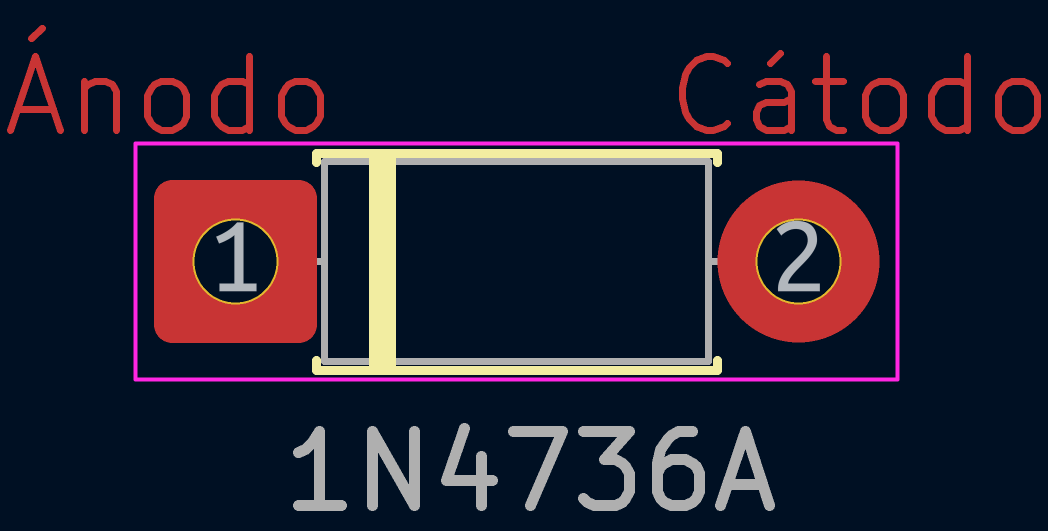
\includegraphics[width=0.4\linewidth]{Imágenes/Prototipo/Diodo KiCad.png}
    \caption{Huella del diodo \textit{zener} utilizada en \textit{KiCad}.}
    \label{fig:zener_kicad}
\end{figure}

Siendo un elemento de protección, no tiene un rol activo en el funcionamiento del circuito, es más, si todo se desarrolla correctamente nunca debería actuar. Pero el hecho que se encuentre en directa conduciendo cuando no debería provocó valores altos de tensión en el nodo del \textit{gate} de los N-MOSFET cuando el sistema está apagado.

[PONER DIAGRAMA DE LA MALLA DEL CIRCUITO Y COMPLETAR]
[ESTA BIEN DECIR QUE LA TENSION ERA DE 3.3-0.7 EN EL GATE CUANDO ESTABA APAGADO?]

Por otro lado, se tiene la huella de los P-MOSFET. Aunque técnicamente era la huella correcta, la hoja de datos da un comentario que no se tuvo en cuenta. En la figura \ref{fig:pmos_config_datasheet} se ve que hay una región que debería estar libre de cobre en la placa, indicada como "KEEP OUT AREA".

\begin{figure}[H]
    \centering
    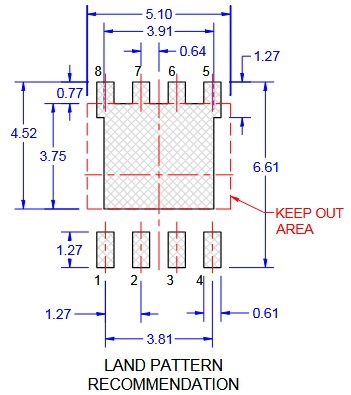
\includegraphics[width=0.5\linewidth]{Imágenes/Prototipo/PMOSFET huella datasheet.jpg}
    \caption{Vista inferior del transistor P-MOSFET FDMS6681Z mostrada en su \textit{datasheet}.}
    \label{fig:pmos_config_datasheet}
\end{figure}

Al no incorporar esa zona, hubieron complicaciones al momento de soldarlo: hicieron falta varios intentos de soldar y desoldar el transistor para evitar que el \textit{drain} entre en cortocircuito con el plano de tierra. Finalmente, lo que se decidió hacer es con un destornillador raspar parte del cobre y así evitar que entre en contacto con el MOSFET, como se muestra en la figura \ref{fig:pmos_arreglado}.

\begin{figure}[H]
    \centering
    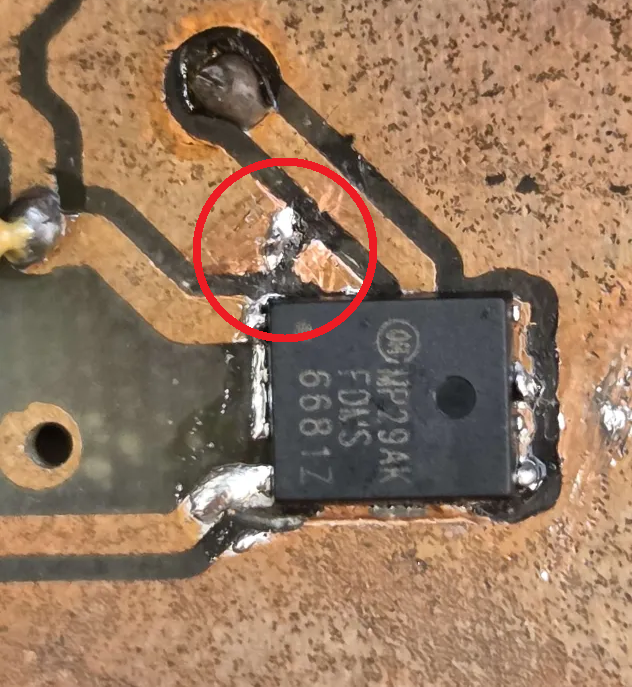
\includegraphics[width=0.4\linewidth]{Imágenes/Prototipo/PMOS arreglado.png}
    \caption{Foto del transistor P-MOSFET FDMS6681Z soldado indicando la corrección que se hizo para que no haya cortocircuito entre el \textit{drain} y el plano de tierra.}
    \label{fig:pmos_arreglado}
\end{figure}

Al margen de los errores de huellas, hubo otro error menor de diseño con el \textit{jumper} del primer banco. Recordemos que se incorporaron \textit{jumpers} para cada banco, de forma que se pueda medir por separado cada uno usando siempre la misma bornera como salida para colocar carga. Sin embargo, para el primer banco, fue mal diseñado como se aprecia en la figura \ref{fig:jumper_mal}.

\begin{figure}[H]
    \centering
    \begin{subfigure}{0.45\textwidth}
        \centering
        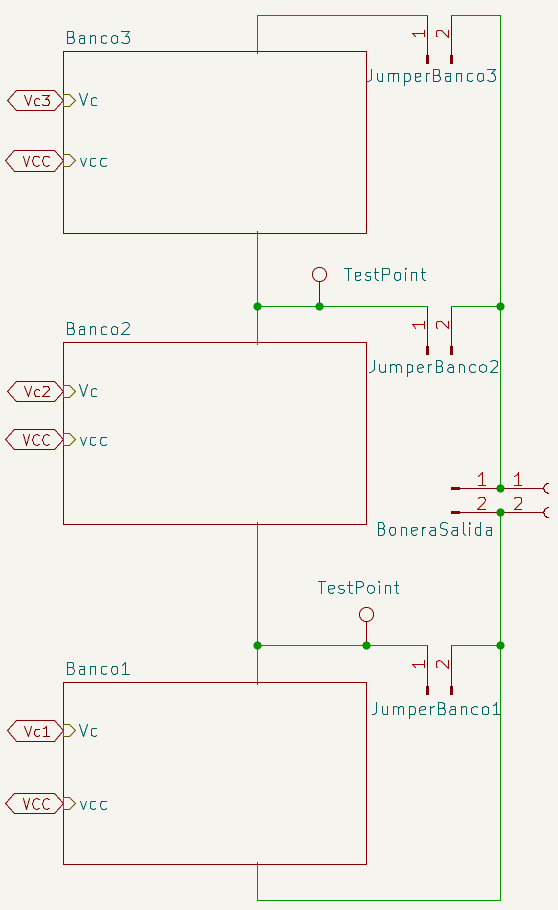
\includegraphics[width=\linewidth]{Imágenes/Prototipo/Jumper Mal.png}
        \caption{}
        \label{fig:jumper_mal}
    \end{subfigure}
    \hfill
    \begin{subfigure}{0.45\textwidth}
        \centering
        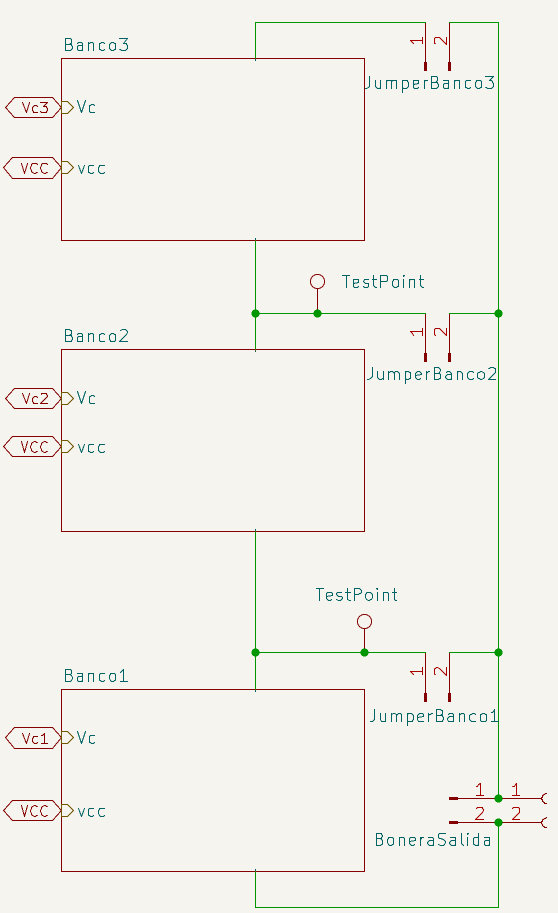
\includegraphics[width=\linewidth]{Imágenes/Prototipo/Jumper Corregido.png}
        \caption{}
        \label{fig:jumper_bien}
    \end{subfigure}
    \caption{Esquema de cómo fue diseñado el circuito prototipo erróneamente en \textit{KiCad} (a) y cómo debería haber sido (b).}
    \label{fig:jumpers}
\end{figure}

El objetivo de los \textit{jumpers} era poder seleccionar si la tensión de la bornera de salida correspondía a una de tres opciones: solo el banco 1, los bancos 1 y 2, o los tres bancos. Sin embargo, como fue diseñado el circuito, el \textit{jumper} correspondiente al primer banco no tenía función alguna, y, en caso que se conecte, se estaría poniendo peligrosamente en cortocircuito a las celdas.

Otro inconveniente fue la forma en la que se soldaron los transistores N-MOSFET. Con el objetivo de minimizar el uso de vías, se utilizaron algunos de los componentes THT para conectar pistas entre capas opuestas. Esto fue práctico usando resistores y diodos pero no fue buena idea con los transistores. Debido a tener pines gruesos, a la forma del encapsulado y a la ubicación en la placa, soldar en la capa \textit{front} resultó incómodo. Como consecuencia de esto, las soldaduras quedaron desprolijas y se torna complicado el proceso de desoldado si fuera necesario.

Por último, el mayor problema que tuvo la placa fue una pobre elección de P-MOSFET como \textit{switch} del circuito \textit{by-pass} de banco. Cuando el transistor debía estar encendido, la tensión $V_{GS}$ era de alrededor de $\SI{1.8}{\volt}$, sin embargo, la tensión de umbral típica (extraída de su hoja de datos) es de $\SI{1.7}{\volt}$. Esto quiere decir que, aunque tecnicamente el MOSFET estaba conduciendo, lo hacía con una resistencia $R_{DS}$ alta entre \textit{drain} y \textit{source}. Es por esto que se veían valores más bajos de lo esperado en la salida: unos $\SI{400}{\milli\volt}$ caen en cada uno de estos transistores cuando están encendidos. Es por esto que se decidió cambiarlo para el circuito final.




Problemas que recordamos:
    - X Huella JFET (corto en la fuente de tensión)
    - X Huella PMOS (corto de drain con tierra)
    - X Huella del Zener (casualidad)
    - X Jumper del banco 1 esta mal puesto
    - X NMOS con soldaduras en las dos capas
    - El PMOS no era correcto
Seguir investigando:
    - Zener funciona raro (no permite que el gate llegue a 0V)
            





